\chapter{Poincar\'e Recurrences, Magnetization, and the First Ising Step}

We begin by going back to the second law, not to weaken it, but to ask in what sense it is compatible with reversible microscopic laws. The lecture starts with a gas in half a room, pushes that puzzle into phase space, and then lets the same line of thought open out into cosmology, Boltzmann brains, and the low-entropy past. Only after that does it reset and turn to magnets: first qualitatively, then through the simplest spin model in an external field, and finally toward the one-dimensional Ising model. These companion notes follow Leonard Susskind's lecture closely, within a chapter-building workflow supported by LazyingArt LLC and Video2Book.

\section{Poincar\'e Recurrences and the Return of Rare States}

Suppose we prepare an absurd initial condition: all the air in the room is placed in the left half. We remove the partition, let the system evolve, and of course the gas spreads out until it looks uniform. Entropy increases. But the lecture does not stop there. It asks the sharper question: if we wait long enough, can the system fluctuate back into the unlikely state with all the molecules once again on one side of the room?

That return of an unlikely macrostate is what we call a Poincar\'e recurrence. Susskind's first point is that this is not mysterious in kind. It is like tossing a coin an enormous number of times and eventually seeing a fantastically unlikely run. The recurrence is not impossible; it is merely rare. The real question is therefore not whether it happens, but how long one must wait.

This is exactly the right place to ask for a timescale. Is the answer a year? A hundred years? The age of the universe? Or something even more extreme? The lecture now turns to phase space in order to make that estimate.

\section{Phase Space, Volume Fractions, and Exponential Waiting Times}

The system lives in phase space, the space of all positions and momenta. For a gas of \(N\) particles this is a very high-dimensional space, of dimension \(6N\): three position coordinates and three momentum coordinates for each particle. Susskind first emphasizes that the momentum directions are bounded once the total energy is bounded, and then, for the counting argument, suppresses momentum and keeps the spatial part of the problem in view.

\begin{figure}
\centering

\includegraphics[width=0.72\textwidth]{lecture_08_figure_02.png}
\caption{Board sketch of a bounded phase-space region with a tangled trajectory. The lecture uses this picture only schematically, as a way of visualizing chaotic wandering through an allowed region.}
\end{figure}

\begin{figure}
\centering
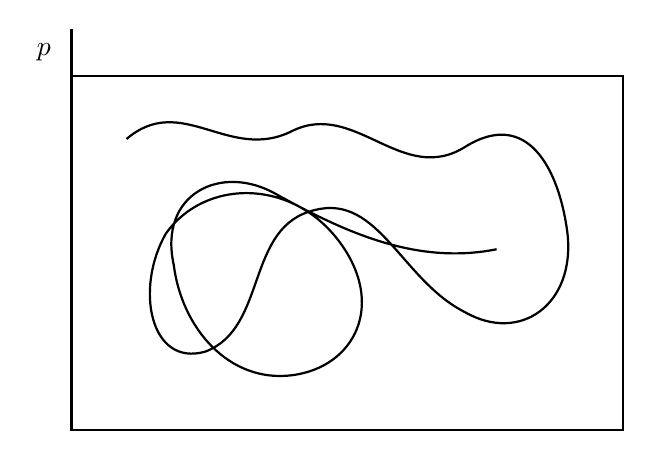
\begin{tikzpicture}[scale=1.0]
\draw[thick] (0,0) rectangle (7,4.5);
\draw[thick] (0,0) -- (0,5.1);
\node at (-0.35,4.8) {\(p\)};
\draw[thick] (0.7,3.7) .. controls (1.4,4.3) and (2.0,3.4) .. (2.8,3.8)
                    .. controls (3.6,4.2) and (4.2,3.1) .. (5.0,3.6)
                    .. controls (5.8,4.1) and (6.2,3.3) .. (6.3,2.5)
                    .. controls (6.4,1.6) and (5.7,1.1) .. (5.0,1.5)
                    .. controls (4.2,1.9) and (3.9,3.0) .. (3.1,2.8)
                    .. controls (2.2,2.6) and (2.5,1.3) .. (1.7,1.0)
                    .. controls (1.0,0.8) and (0.8,1.8) .. (1.2,2.5)
                    .. controls (1.7,3.2) and (2.8,3.2) .. (3.4,2.4)
                    .. controls (4.0,1.6) and (3.6,0.8) .. (2.8,0.7)
                    .. controls (2.0,0.6) and (1.4,1.3) .. (1.3,2.1)
                    .. controls (1.1,3.0) and (1.9,3.4) .. (2.6,3.0)
                    .. controls (3.5,2.5) and (4.4,2.1) .. (5.4,2.3);
\end{tikzpicture}
\caption{A clean redraw of the same schematic. The point is only that chaotic motion can wind through the accessible region in a very complicated way.}
\end{figure}

The first picture is deliberately misleading if we take it too literally. If the accessible region is split into left and right halves, then in a two-dimensional drawing it looks as if the system would spend half its time in the left half. That cannot be the right answer for a gas returning to one side of a room. The mistake is that the physically relevant condition is not that one coordinate lies in one half, but that \emph{all} of them do.

So let us strip the problem down further. Ignore momentum and imagine only two particles moving in one dimension. Their configuration is described by two coordinates, say \(x_1\) and \(x_2\). The full configuration space is a square. The condition that both particles lie in the left half of the room picks out one quarter of that square. Therefore the relevant fraction of configuration space is
\begin{equation}
P_2=\frac{1}{4}.
\end{equation}
For three particles the same logic gives \(2^{-3}\), and for \(N\) particles,
\begin{equation}
P_{\mathrm{half}}(N)=\left(\frac{1}{2}\right)^N.
\end{equation}

This is the first serious correction to low-dimensional intuition. The suppression is not merely geometric in two dimensions; it is exponential in the number of particles.

Susskind then broadens the argument. Suppose the particles are required to lie not merely in half the room, but in some smaller spatial region of volume \(v\) inside a box of volume \(V\). Ignoring momentum for the estimate, the full configuration-space volume scales like \(V^N\), while the special subregion scales like \(v^N\). Hence the fraction of time spent there is
\begin{equation}
P(v)=\frac{v^N}{V^N}=\left(\frac{v}{V}\right)^N.
\end{equation}
The recurrence time is then estimated by the inverse small probability,
\begin{equation}
\tau_{\mathrm{rec}} \sim \frac{1}{P(v)} \sim \left(\frac{V}{v}\right)^N.
\end{equation}
For the half-room example this becomes
\begin{equation}
\tau_{\mathrm{rec}} \sim 2^N.
\end{equation}

The lecture then translates the same statement into entropy language. Since the entropy of a region of phase space is the logarithm of its volume, the equilibrium region has exponentially large volume compared with any sharply localized region. Schematically one may write
\begin{equation}
P \sim e^{-S_{\mathrm{eq}}},
\end{equation}
with the understanding that this is a coarse statement about scaling, not a carefully normalized theorem. The real point is that for room-sized numbers of molecules, \(N\) is so large that \(2^N\) becomes absurdly large. Susskind emphasizes numbers of the form \(2^{10^{30}}\): a number so far beyond ordinary timescales that practical language ceases to matter.

\subsection{Question \& Answer}

\paragraph{Question.} Does the unit of time matter? If the recurrence time is given in seconds, might it become less absurd in hours, or in some still shorter unit?

\paragraph{Answer.} On any human scale, no. If
\begin{equation}
\tau_{\mathrm{rec}} \sim 2^{10^{30}}
\end{equation}
in one unit, then converting to another unit only divides by some finite conversion factor such as \(3600\). That changes the number by a multiplicative constant, but it does not touch the fact that the exponent is of order \(10^{30}\). The lecture's point is precisely that once the estimate is this extreme, the choice of seconds, hours, or years is conceptually irrelevant. What does depend on microscopic details is how long the system actually lingers in the special corner when it gets there; the recurrence estimate concerns how rarely it returns, not the detailed duration of the visit.

\section{Reversibility, Low-Entropy Initial Data, and Boltzmann Brains}

At this point the lecture changes register. The raw number is not the point by itself. The point is that it reconciles microscopic reversibility with thermodynamic one-wayness.

A truly closed system, watched for a sufficiently long time, does not only move from odd states to ordinary-looking equilibrium states. It also fluctuates back. Over times comparable to the recurrence time, oddness goes up and down in a time-symmetric way. In that sense the microscopic laws remain reversible.

What is \emph{not} time-symmetric is our choice of initial condition. If we knowingly begin in a very special, tiny corner of phase space, then the overwhelmingly likely next step is to leave that corner. That is the content of the second law as it is actually used. The law is not contradicted by reversibility; it depends on the fact that the world begins in an extraordinarily unrepresentative state.

This is exactly where the lecture turns outward to cosmology. If the universe really began in a low-entropy state, why did it do so? Boltzmann understood that recurrence by itself does not answer that question. It only shifts the puzzle. A recurrence estimate tells us that rare states recur in a closed system, but it does not explain why the world we inhabit looks as though it emerged from a coherent low-entropy past rather than from a small random fluctuation inside equilibrium.

\subsection{Question \& Answer}

\paragraph{Question.} If a closed system recurs forever, why not say that we are simply one random fluctuation? Why not explain the observed world that way?

\paragraph{Answer.} Because a random fluctuation predicts the wrong kind of world. If one asks for the most probable fluctuation compatible with the existence of observers, then one does not get a structured cosmos full of stars, galaxies, mutually consistent records, and a long coherent history. One gets the \emph{smallest} fluctuation that is sufficient to produce the observer.

This is the force of the Boltzmann-brain discussion. A single planet is enormously unlikely. Two planets are vastly more unlikely. A whole sky full of correlated astronomical structure is more unlikely still. If one imagines a fluctuation that produces a lone observer, then the conditional probability of also finding an elaborate external world is tiny. Susskind drives the point home with deliberately sharp examples: if a ``Boltzmann head'' fluctuates into existence, the probability that the rest of its life, family, and environment are also present is much smaller than the probability of the head alone.

The lecture then names the deeper problem: \emph{historical coherence}. In the world we actually observe, records agree with one another. Textbooks, fossils, observations, and memories all point to a mutually consistent past. A pure fluctuation theory does not naturally explain that. If the present state were assembled at random, there would be no good reason for different records to line up into a coherent history. That is why recurrence, though real as a conceptual point, is not a satisfactory statistical explanation of the world as we see it.

\section{Why Life Does Not Violate the Second Law}

The next conceptual obstacle is equally natural. If entropy tends to increase, how can life sustain organized structure for long times? The lecture answers this directly and refuses the premise that life is a counterexample.

\subsection{Question \& Answer}

\paragraph{Question.} Does life decrease entropy?

\paragraph{Answer.} Not for the whole system. The second law does not say that every subsystem must increase its entropy at every moment. It says that any local decrease must be paid for by a greater increase elsewhere.

The key distinction here is between equilibrium and a stationary nonequilibrium state. The Earth is not an isolated system in equilibrium. It is a system through which energy flows. That flow supports structure. Susskind's analogy is a pipe with water running through it. The flow can generate vortices and eddies. Those structures are not violations of mechanics or thermodynamics; they are precisely the kinds of organized patterns that sustained flow can create. If the ends of the pipe are sealed, the flow stops, the vortices disappear, and the system relaxes to dull equilibrium.

Life, in this picture, is an eddy in an energy flow. The relevant flow for Earth is solar radiation. If sunlight were cut off and no energy exchange were allowed, the Earth would eventually settle into featureless thermal equilibrium. So life is not a loophole in the second law. It is a nonequilibrium structure maintained by throughput.

\section{From Real Magnets to the Simplest Spin Model}

After that long detour through interesting things, the lecture says, in effect: back to dull things. Magnets.

Susskind begins physically. A real magnet is made from many little magnets, perhaps as small as atomic moments, perhaps larger as grains or domains. At very high temperature these microscopic moments are randomly oriented, so there is no net magnetization. As the temperature is lowered, the energy may favor local alignment. Small groups begin to align, producing domains. If the temperature is lowered still further, those domains may grow until a macroscopic magnetic orientation appears. That appearance of global order is a magnetic phase transition.

At zero temperature the intuition is straightforward: the Boltzmann distribution concentrates on the lowest-energy state, so if alignment lowers the energy, one expects all the moments to line up. But in which direction? That question already hints at spontaneous symmetry breaking. There may be no externally imposed preferred direction, and yet the ordered phase chooses one.

The lecture then strips the model down radically. We do not allow the little magnets to point in arbitrary directions. Each one points only up or down. This is not realism; it is a deliberate simplification.

Let there be \(N\) such spins, and let
\begin{equation}
\sigma_i=\pm 1
\end{equation}
encode whether the \(i\)-th spin is up or down. The first model has no interaction between spins at all. Instead, there is an external magnetic field \(H\), and each spin has magnetic moment \(\mu\). The board equations make the chosen sign convention clear: with the field oriented so that down is energetically preferred, an up spin has energy \(+\mu H\) and a down spin has energy \(-\mu H\).

\begin{figure}
\centering

\includegraphics[width=0.78\textwidth]{lecture_08_figure_03.png}
\caption{Board setup for the noninteracting spin model in an external field. The lecture first fixes the counting variables \(n\) and \(m\), then writes the total energy.}
\end{figure}

If \(n\) spins are up and \(m\) spins are down, then
\begin{equation}
n+m=N,
\end{equation}
and the total energy is
\begin{equation}
E=(n-m)\mu H.
\end{equation}
That is the first complete energy function of the magnetic part of the lecture, and once it is written we can do statistical mechanics.

\section{Independent Spins in an External Field}

The next step is combinatorics. For fixed \(n\) and \(m\), how many distinct configurations are there? We are choosing which \(n\) of the \(N\) spins point up, so the multiplicity is
\begin{equation}
\Omega(n,m)=\frac{N!}{n!\,m!}.
\end{equation}
This gives the number of states with the same energy \(E=(n-m)\mu H\).

\begin{figure}
\centering

\includegraphics[width=0.78\textwidth]{lecture_08_figure_04.png}
\caption{Board stage of the partition-function derivation. The screenshot is useful for order and layout; the cleaned algebra below supplies the legible calculation.}
\end{figure}

Now we write the partition function. The lecture first writes it schematically as a sum over configurations, and then uses the multiplicity to collapse the sum onto the counting variables:
\begin{align}
Z
&=\sum_{n+m=N} \Omega(n,m)\,e^{-\beta \mu H (n-m)} \\
&=\sum_{n=0}^{N} \frac{N!}{n!(N-n)!}
\left(e^{-\beta\mu H}\right)^n
\left(e^{+\beta\mu H}\right)^{N-n}.
\end{align}
At this stage Susskind introduces the temporary abbreviations
\begin{equation}
x=e^{-\beta\mu H},
\qquad
y=e^{+\beta\mu H}.
\end{equation}
Then
\begin{align}
Z
&=\sum_{n=0}^{N}\frac{N!}{n!(N-n)!}\,x^n y^{N-n} \\
&=(x+y)^N \\
&=\left(e^{-\beta\mu H}+e^{+\beta\mu H}\right)^N \\
&=2^N\cosh^N(\beta\mu H).
\end{align}
The transcript is garbled around the \(x,y\) step, but the board structure and the binomial theorem make the intended derivation clear.

Before differentiating anything, the lecture defines magnetization. The first statement is slightly corrected on the fly, and the corrected definition is the one we keep:
\begin{equation}
M=\left\langle \frac{n-m}{N}\right\rangle.
\end{equation}
This is the average excess of up over down spins per site. It is naturally related to the energy through
\begin{equation}
\langle E\rangle = N\mu H\,M.
\end{equation}

\begin{figure}
\centering

\includegraphics[width=0.78\textwidth]{lecture_08_figure_05.png}
\caption{Board emphasis on the corrected magnetization definition and the energy--magnetization relation. The lecture pauses here to clarify that the physically relevant quantities are Boltzmann averages.}
\end{figure}

\subsection{Question \& Answer}

\paragraph{Question.} Is magnetization here a property of one configuration, or are we speaking about an average magnetization?

\paragraph{Answer.} In statistical mechanics we are speaking about an average over the Boltzmann distribution. Configuration by configuration, the quantity \((n-m)/N\) measures the spin excess for that state. The observable magnetization is the Boltzmann average of that quantity. The same goes for the energy. If
\[
E=(n-m)\mu H
\]
holds for each configuration, then averaging both sides gives
\[
\langle E\rangle = N\mu H \left\langle \frac{n-m}{N}\right\rangle = N\mu H\,M.
\]
This is the clarification the lecture insists on before moving on.

With that settled, the average energy follows from the standard thermodynamic identity
\begin{equation}
\langle E\rangle = -\frac{\partial}{\partial \beta}\log Z.
\end{equation}
Using
\begin{equation}
Z=2^N\cosh^N(\beta\mu H),
\end{equation}
we have
\begin{equation}
\log Z = N\log 2 + N\log\!\bigl(\cosh(\beta\mu H)\bigr),
\end{equation}
and so
\begin{align}
\langle E\rangle
&=-\frac{\partial}{\partial \beta}\log Z \\
&=-N\mu H \,\frac{\sinh(\beta\mu H)}{\cosh(\beta\mu H)} \\
&=-N\mu H\,\tanh(\beta\mu H).
\end{align}
Therefore
\begin{equation}
M = \frac{\langle E\rangle}{N\mu H}
= -\tanh(\beta\mu H).
\end{equation}

This is the complete solution of the simple model. It is also a good place to stop and think. At zero temperature, \(\beta\to \infty\), so \(\tanh(\beta\mu H)\to 1\), and therefore
\begin{equation}
M \to -1.
\end{equation}
All spins point down, as expected from the bias in the external field. At infinite temperature, \(\beta\to 0\), so
\begin{equation}
M \to 0.
\end{equation}
Thermal randomness defeats the weak energy preference. If we reverse the magnetic field, \(H\to -H\), the sign of the magnetization reverses as well.

The lecture spends time on these limits because they are the physical content of the formula. The result is not just an algebraic expression. It tells us how a biased two-state system interpolates smoothly from full alignment at low temperature to no net magnetization at infinite temperature. And precisely because the field explicitly biases one direction over the other, there is no symmetry here and no phase transition. That is why the lecture is now ready to move to the Ising model.

\section{The First Ising Step: Neighbor Interactions, Symmetry, and Next Time}

The previous model is too simple to display the phenomenon we really want. The external field already picks a preferred direction, so the model has no up-down symmetry. The first Ising step restores that symmetry by removing the external field and putting the energy into the interaction between neighboring spins.

\begin{figure}
\centering

\includegraphics[width=0.72\textwidth]{lecture_08_figure_06.png}
\caption{The first Ising interaction as written on the board. The key point is the minus sign: aligned neighboring spins are assigned lower energy.}
\end{figure}

The lecture first focuses on a pair of neighboring spins. If one wrote \(J\sigma_{(1)}\sigma_{(2)}\), then anti-aligned spins would have lower energy. Susskind wants the opposite convention, so he inserts a minus sign:
\begin{equation}
E_{12}=-J\,\sigma_{(1)}\sigma_{(2)},
\qquad J>0.
\end{equation}
Thus aligned spins have lower energy and anti-aligned spins have higher energy.

\begin{figure}
\centering
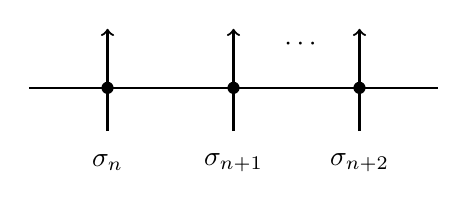
\begin{tikzpicture}[scale=1.0]
\draw[thick] (0,0) -- (5.2,0);
\fill (1,0) circle (2.2pt);
\fill (2.6,0) circle (2.2pt);
\fill (4.2,0) circle (2.2pt);
\draw[->,thick] (1,-0.55) -- (1,0.75);
\draw[->,thick] (2.6,-0.55) -- (2.6,0.75);
\draw[->,thick] (4.2,-0.55) -- (4.2,0.75);
\node at (1,-0.95) {\(\sigma_n\)};
\node at (2.6,-0.95) {\(\sigma_{n+1}\)};
\node at (4.2,-0.95) {\(\sigma_{n+2}\)};
\node at (3.45,0.55) {\(\cdots\)};
\end{tikzpicture}
\caption{Minimal redraw of the nearest-neighbor interaction along a line. The lecture extends the two-spin rule by summing each neighboring pair once.}
\end{figure}

For a chain of spins on a one-dimensional lattice, the energy becomes
\begin{equation}
E=-J\sum_n \sigma_n \sigma_{n+1}.
\end{equation}
This Hamiltonian has a global spin-flip symmetry:
\begin{equation}
\sigma_i \mapsto -\sigma_i
\qquad \text{for all } i.
\end{equation}
Every configuration has a partner with all spins reversed and with exactly the same energy. That is the mathematical statement of the up-down symmetry.

The lecture uses this to distinguish sharply between the simple field-biased model and the Ising model. In the field-biased model, there is no symmetry to break. In the Ising model there is, and so if magnetization appears, it must come from spontaneous symmetry breaking.

One can already discuss the limiting cases. At infinite temperature, everything is random. The average magnetization vanishes, and the average nearest-neighbor product vanishes as well:
\begin{equation}
\langle \sigma_n \sigma_{n+1}\rangle = 0
\qquad (T=\infty).
\end{equation}
Hence the average energy is zero relative to the convention of the Hamiltonian, even though the ground state energy is negative. This was one of the lecture's nice clarifications: zero energy here means high energy relative to the aligned ground state.

At zero temperature the situation is different. The energy is minimized when all neighboring pairs are aligned. In one dimension there are therefore two ground states,
\begin{equation}
(\uparrow \uparrow \uparrow \cdots \uparrow)
\qquad \text{and} \qquad
(\downarrow \downarrow \downarrow \cdots \downarrow).
\end{equation}
They have equal energy. The symmetry does not tell the system which one to choose.

Now add the tiniest stray magnetic field acting on even a single site. At strictly zero temperature, the Boltzmann distribution selects the true lowest-energy state infinitely strongly. That infinitesimal bias can therefore choose one orientation for the whole chain. If the field is then removed, the ordered state may persist because each spin is held in place by its neighbors. This is the lecture's entry point to spontaneous symmetry breaking.

The lecture stops here deliberately. The model is now posed, but not yet solved. The next job is to compute its partition function and see what really happens in one dimension. The answer, previewed at the end of the lecture, is that the one-dimensional Ising model has no finite-temperature phase transition. The first truly interesting case is the two-dimensional model.

\section{Summary}

The chapter began by returning to the second law through the concrete puzzle of recurrence. A gas prepared in an unlikely macrostate will almost certainly spread out, but in a closed system it will also recur after an exponentially long time. The relevant suppression is not low-dimensional geometry but high-dimensional counting:
\[
P \sim \left(\frac{v}{V}\right)^N \sim e^{-S_{\mathrm{eq}}},
\qquad
\tau_{\mathrm{rec}} \sim P^{-1}.
\]
That estimate explains how microscopic reversibility and thermodynamic one-wayness coexist, while leaving intact the deeper question of why the universe began in a low-entropy state.

The lecture then used that same statistical way of thinking to motivate magnets. In the simplest spin model with an external field, one can count configurations exactly, derive
\[
Z=2^N\cosh^N(\beta\mu H),
\]
and from it obtain
\[
M=-\tanh(\beta\mu H).
\]
That model is biased and therefore has no phase transition. The Ising model removes the bias, places the energy in neighboring pairs, restores a global spin-flip symmetry, and sets the stage for the real question: when can a symmetric interacting system choose an ordered state on its own?